\documentclass[12pt, letterpaper, twoside]{article}
\usepackage{amsmath}
\usepackage{url}
\usepackage[utf8]{inputenc}
\usepackage[ukrainian]{babel}
\usepackage{graphicx}
\title{Проєкт з дискретної математики: 
	Алгоритм Борувки}
\author{Автори проєкту: Кирило Шихальов (ДМ 4) та Олексій Степаник (ДМ 4)}
\date{\today}

\begin{document}
\maketitle
\section{Формальний опис алгоритму}
\subsection{Основні задачі}
Наш алгоритм є жадібним, неорієнтованим і зважаним. Головною задачею є пошук мінімального кістякового дерева в зваженому зв'язному графі.

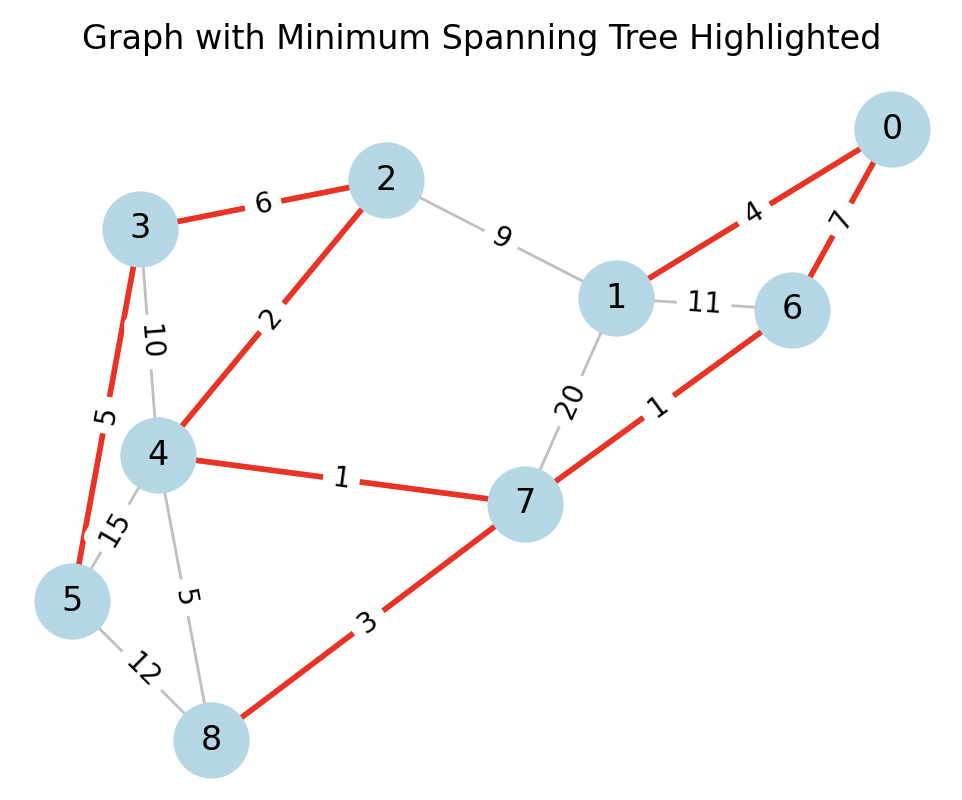
\includegraphics{graph.png}
\subsection{Вхідні та вихідні дані}
Вхідні дані - зважений зв'язний граф, представлений як набір вершин та ребер, кожне з яких має вагу. Вихідні дані - мінімальне кістякове дерево, яке з'єднує всі вершини без циклів з мінімальною сумою ваг.

\subsection{Алгоритм}
\begin{verbatim}	
	function Boruvka(G):
	input: graph G with weights on edges
	output: minimum spanning tree T
	for each vertex v in G:
		create a set {v}
	T = empty graph with the same vertices as G
	while T has fewer than n-1 edges:
		for each set S in the set of sets:
			find the edge e with the smallest weight that connects S with a vertex outside S
	if e does not create a cycle in T:
		add e to T
	unite the sets that e connect
	
	return T
\end{verbatim}
\subsection{Просторові оцінки}
Часова складність: \(O(E\log V)\), де \(E\) - кількість ребер, а \(V\) - кількість вершин. Просторова складність: \(O(V+E)\).

\section{Програмна реалізація,(коменатарі до неї)}


Наш алгоритм працює за принципом створення 
графу і згодом пошук мінімального кістякового дерева.
Спочатку ми зробили реалізацію неорієнтованого графу з вершинами та ребрами. Кожна вершина має суміжні вершини та список ребер, до яких вона належить. Кожне ребро має два кінцеві вершини та вагу. В об’єкті Graph ми зробили список, який містить в собі вершини та ребра. Він має усі методи роботи з графом, наприклад такі, як додавання та видалення вершин, ребер, а також для перевірки суміжності двох вершин. Також реалізовані методи для отримання списку суміжності вершини та перетворення графу в матрицю суміжності. 
Обрано такі рішення та типи даних:
Використано класи Vertex та Edge для представлення вершин та ребер відповідно. Кожен клас містить необхідні поля та конструктори.
Vertex: Репрезентує вершину в графі. Кожна вершина має ім'я, список сусідів і список ребер.
Edge: Репрезентує ребро в графі. Кожне ребро з'єднує дві вершини і має вагу.
Для представлення графу використано клас Graph, який містить список вершин та ребер. Використання списків дозволяє легко маніпулювати вершинами та ребрами графу.
В ціломую Код використовує клас List із .NET Framework для зберігання вершин і ребер, що забезпечує функціональність динамічного масиву та амортизований час доступу O(1), звичайно ми також могли щроиби і через Hash, але вибрали працювати з лістами, бо мають більший функціонал . У гіршому випадку методи Add і Remove зі списку мають час виконання O(n), але це прийнятно для використання за призначенням.
Також були створені два методи перший з яких це \textbf {AdjacencyList} він повертає список списків сусідів, де кожен внутрішній список містить сусідів вершини. Це представлення дозволяє ефективну ітерацію сусідів вершини з часом виконання O(deg(v)) для вершини ступеня deg(v).
Другий Метод \textbf{AdjacencyMatrix} він повертає двовимірний масив, який представляє графік як матрицю суміжності. Це представлення дає змогу ефективно знаходити ваги ребер між вершинами, а час виконання для доступу до одного запису становить O(1). Але час виконання для створення матриці суміжності дорівнює $O(n^{2})$, де n - кількість вершин.

Загалом, код забезпечує гнучку та ефективну реалізацію структур даних графів.



\section{Посилання на GitHub-репозиторій}
\url{https://github.com/Oleksii-Stepanyk/DM_Project}

\section{Експериментальна частина}
\centering \subsection*{Схема експерименту та обрані параметри}
\begin{flushleft}
	Для проведення чисельних експериментів, нам потрібно визначитись з параметрами, а саме зі щільністю та розмірністю графа.
	Оскільки наш алгоритм шукає мінімальне кістякове дерево графу, найкраще буде перевірити його в умовах, коли ребер багато і степені вершин $\approx$ хоча б половині кількості вершинL
\end{flushleft}

\section{Висновки}

(Тут ваші висновки)

\end{document}
